\section{ CONECTAR A SQL SERVER DESDE POWER BI DESKTOP} 

\begin{itemize}

\item 1. Iniciar Power BI Desktop.
\item 2. Cuando la Ventana de Power BI Desktop aparezca, en el panel a mano izquierda, hacer click en Obtener Datos (Get Data). \\
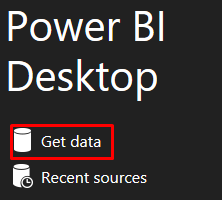
\includegraphics[scale=0.5]{./Imagenes/image001}
\item 3. En el cuadro de dialogo Obtener Datos (Get Data), click en base de datos SQL Server, y luego hacer click en Conectar (Connect) \\
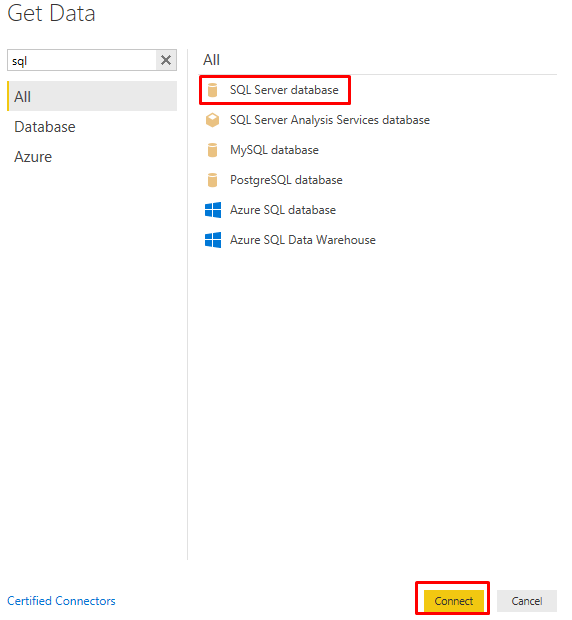
\includegraphics[scale=0.5]{./Imagenes/image002}
\item 4. En el cuadro de dialogo base de datos SQL Server, en la casilla servidor tipear (local), en la casilla Base de datos (opcional) / Database (optional), tipear AdventureWorks2017, y hacer clic en OK. \\
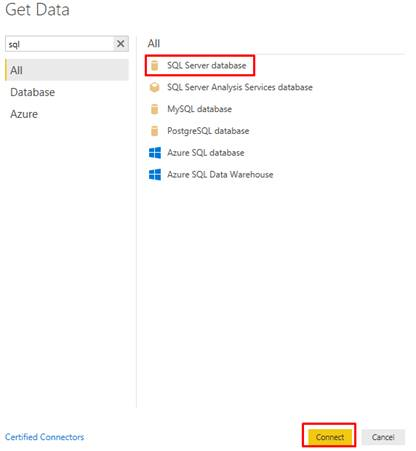
\includegraphics[scale=0.8]{./Imagenes/image003}
\item 5. En el cuadro de dialogo base de datos SQL Server, aceptar los valores por defecto, y luego click en el Conectar (Connect). Si un mensaje de Soporte de Encriptación es visualizado, hacer click en OK. \\
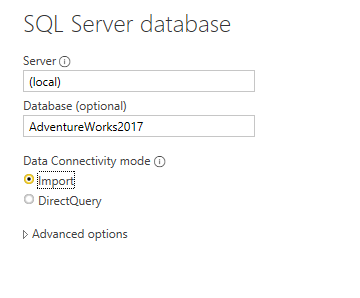
\includegraphics[scale=0.5]{./Imagenes/image004}
\item 6. En el cuadro de dialogo Navegador (Navigator), seleccionar el check en Sales.vSalesPerson, y entonces hacer click en Cargar (Load). \\
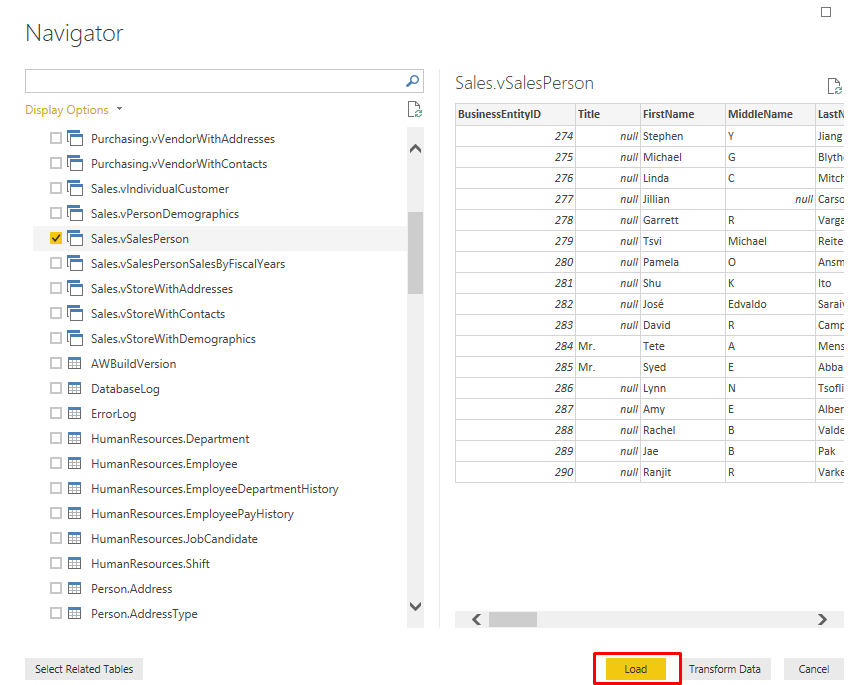
\includegraphics[scale=0.8]{./Imagenes/image005}
\item 7. En el panel Campos (Fields), expandir Sales vSalesPerson para ver todas las columnas. \\
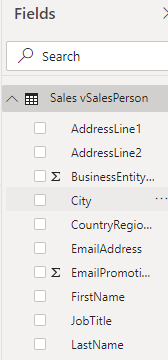
\includegraphics[scale=0.5]{./Imagenes/image006}
\item 8. En el menu principal (Home ribbon), hacer click en Funetes Recientes (Recent Sources), y en local: AdventureWorks2017. \\
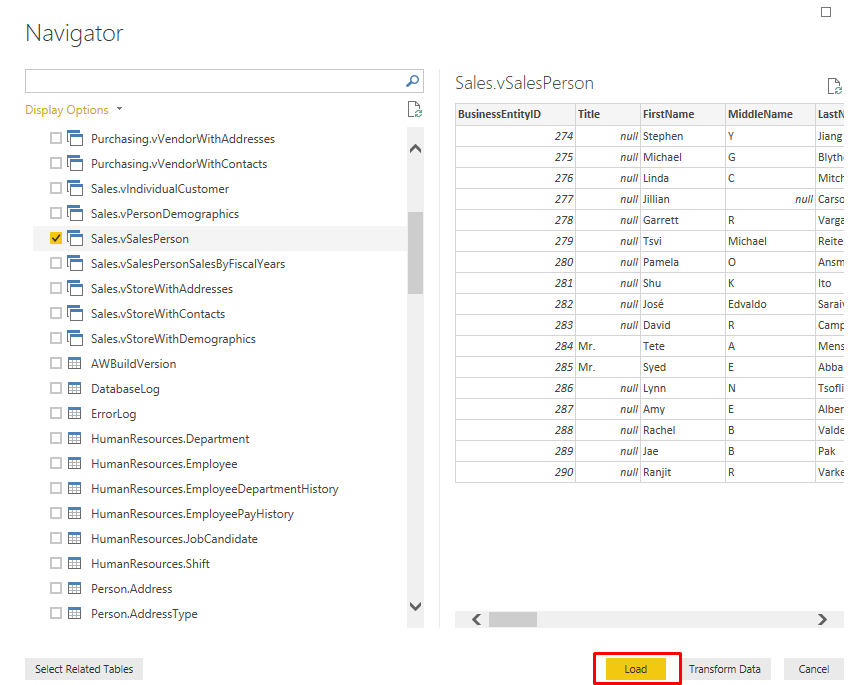
\includegraphics[scale=0.5]{./Imagenes/image007}
\item 9. En el cuadro de dialogo Navegador (Navigator), seleccionar la vista Sales.vStoreWithDemographics, y luego
hacer click en Cargar (Load). \\
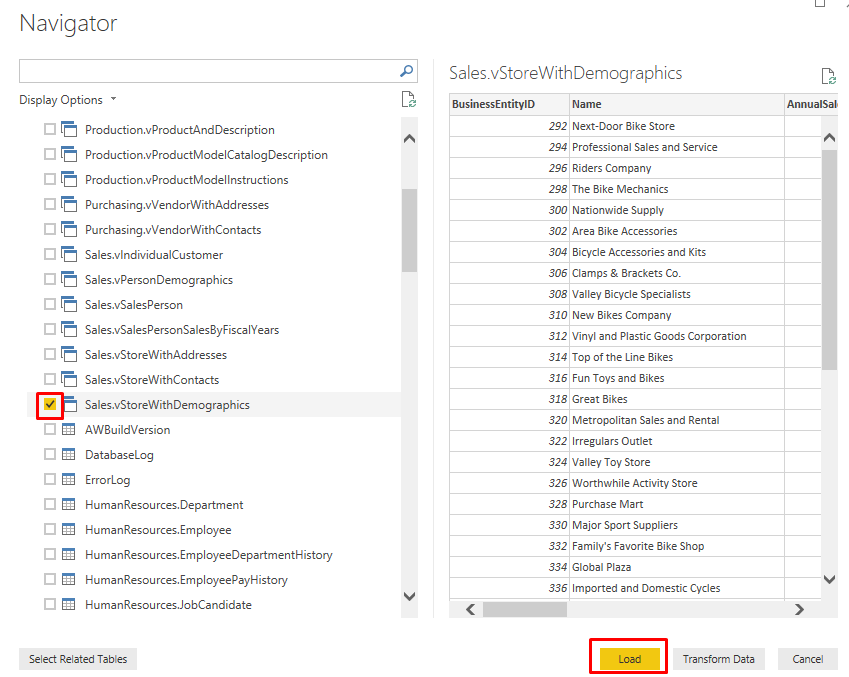
\includegraphics[scale=0.8]{./Imagenes/image008}
\item 10. En el panel Campos (Fields), expandir Sales.vStoreWithDemographics para ver todas las columnas. \\
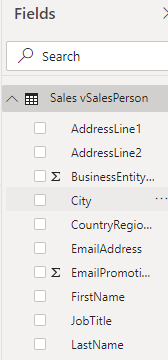
\includegraphics[scale=0.5]{./Imagenes/image009}
\item 11. En el menu principal (Home ribbon), hacer click en Obtener Datos (Get Data), y luego click en SQL Server. \\
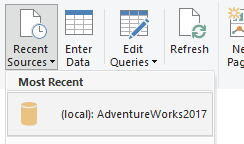
\includegraphics[scale=0.5]{./Imagenes/image010}
\item 12. En el cuadro dialogo base de datos SQL Server, en la casilla Servidor (Server), tipear (local), y en la casilla Base de datos (opcional), tipear AdventureWorks2017. \\
\item 13. Expandir opciones Avanzadas, en la casilla sentencia SQL (opcional, base de datos requerida), tipear la siguiente consulta, y luego hacer click en OK:
\\ SELECT TOP 10 P.ProductID, P.Name AS Product, SUM(CAST(LineTotal AS decimal(18,2))) AS LineTotal FROM
 Purchasing.PurchaseOrderDetail AS POD INNER JOIN Production.Product AS P ON POD.ProductID = P.ProductID \\
GROUP BY P.ProductID, P.Name ORDER BY LineTotal DESC \\ 
\item 14. Si la Ventana Configuración de la Conexión (Connection Settings) aparece, hacer click en OK. \\
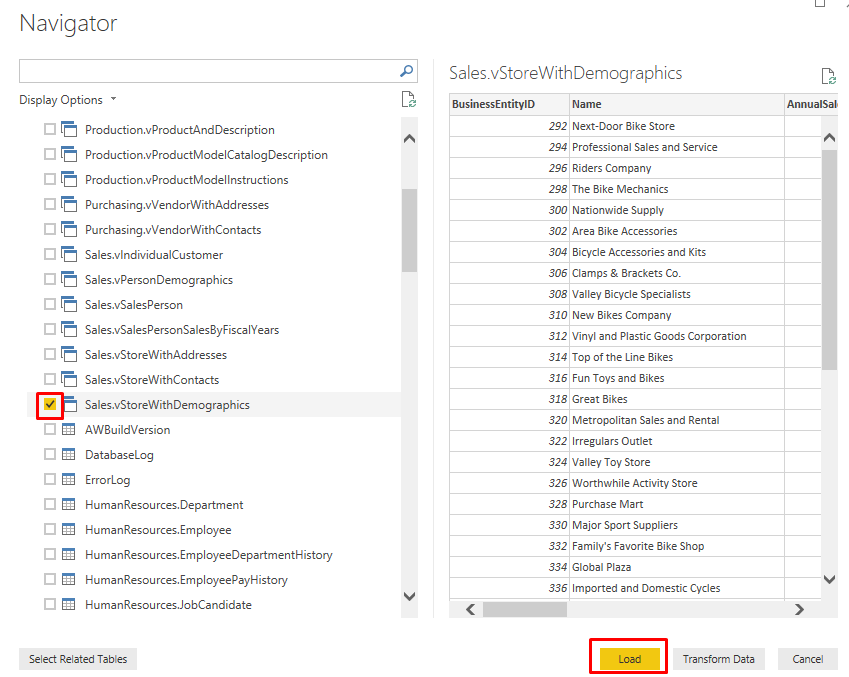
\includegraphics[scale=0.5]{./Imagenes/image011}
\item 15. En el cuadro de dialogo (local): AdventureWorks2017 hacer click en Cargar (Load). \\
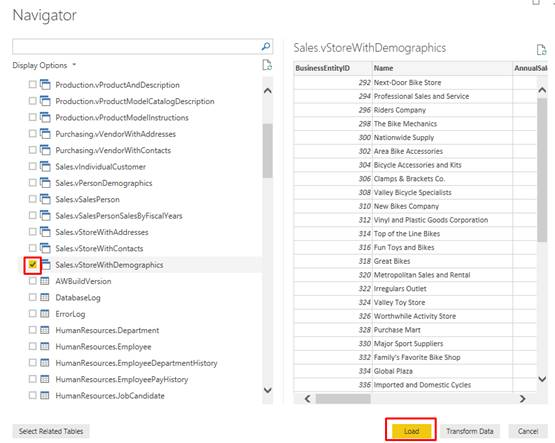
\includegraphics[scale=0.8]{./Imagenes/image012}
\item 16. En el panel Campos, expander Query1 para ver todas las columnas. \\
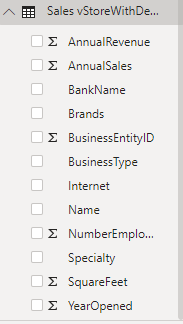
\includegraphics[scale=0.5]{./Imagenes/image013}
\item 17. Hacer click en la elipsis (…) al lado de Query1 y hacer click en Renombrar, tipear Top 10 Producto Vendidos, y presionar Enter. \\
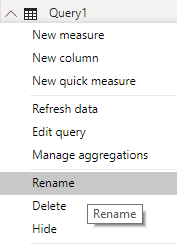
\includegraphics[scale=0.5]{./Imagenes/image014}


\end{itemize}